\documentclass[handout]{ximera}

\title{Practice 2}
\author{A Ximera Author}

\begin{document}

\begin{abstract}
Practice number two!
\end{abstract}


\maketitle

Here's a second sample question.

\begin{problem}
\begin{multipleChoice}
\choice{Incorrect}
\choice{Not this one!}
\choice[correct]{Click here?}
\choice{Not me!}
\choice{Not me either!!}
\end{multipleChoice}
\end{problem}

\begin{problem}
   Evaluate $2 + 3 = \answer{5}$ or that $x \cdot x = \answer{x^2}$.
\end{problem}

\begin{center}
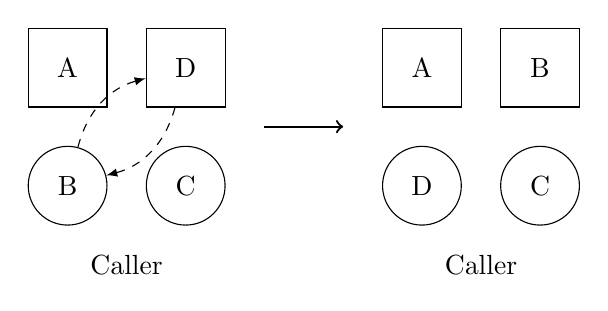
\begin{tikzpicture}
\node[rectangle,draw, minimum size=1cm] (A) at  (-3,.75) {A};
\node[circle,draw, minimum size=1cm] (B) at  (-3,-.75) {B};
\node[circle,draw, minimum size=1cm] (C) at  (-1.50,-.75)  {C};
\node[rectangle,draw, minimum size=1cm] (D) at  (-1.50,.75)  {D};
\node[] at (-2.25,-1.75) {Caller};
     \draw[->, black, thick] (-.5,0) -- (.5,0);
    \draw [thin, dashed, -latex] (B) to [bend left] (D);
    \draw [thin, dashed, -latex] (D) to [bend left] (B);
\node[rectangle,draw, minimum size=1cm] (A) at  (1.5,.75) {A};
\node[rectangle,draw, minimum size=1cm] (B) at  (3,.75) {B};
\node[circle,draw, minimum size=1cm] (C) at  (3,-.75)  {C};
\node[circle,draw, minimum size=1cm] (D) at  (1.5,-.75)  {D};
\node[] at (2.25,-1.75) {Caller};
\end{tikzpicture}
\end{center}

\begin{question}
True or False: My name is Jessica. (This has a drop down menu!) \wordChoice{\choice[correct]{True} \choice{False}}
\end{question}

\geogebra[sdz,stb]{mG34YseZ}{840}{750}




\end{document}